\documentclass[12pt,a4paper]{extarticle}
\usepackage[utf8]{inputenc}
\usepackage[T5]{fontenc}
\usepackage{geometry}
\geometry{a4paper, left=1.5cm, right=1cm, top=1.5cm, bottom=1.5cm, headheight=20pt, headsep=15pt, footskip=28pt}
\usepackage{enumitem}
\usepackage{amssymb}
\usepackage{tikz}
\usetikzlibrary{patterns, patterns.meta} % Thêm patterns.meta vào đây
% Gọi package nằm trong thư mục con template
\usepackage{../template/mngocbox}

\begin{document}

% Sử dụng ngoặc vuông [...] để thay đổi linh hoạt các thông số
\makeheadbox[headerright={Tổng ôn 10-11},chude={CHỦ ĐỀ 04},tieude={Tam thức bậc hai},dinhdang={Đại số},lop={12 },gv={Nguyễn Lê Minh Ngọc}]

\vspace{2em}
\makeheading{I}{Tóm tắt lý thuyết}
\section{Hàm số bậc hai}
\subsection*{1. Khái niệm hàm số bậc hai}
Tổng quát, ta có Hàm số bậc hai là hàm số được cho bởi công thức:
\[ y = ax^2 + bx + c, \]
trong đó $x$ là biến số, $a, b, c$ là những hằng số và $a \neq 0$.
Tập xác định của hàm số bậc hai là $\mathbb{R}$.
\noindent $\blacktriangleright$ \textbf{Nhận xét}: Hàm số $y = ax^2$ ($a \neq 0$) đã học ở lớp 9 là một trường hợp đặc biệt của hàm số bậc hai với $b = c = 0$.
\subsubsection*{2. Đồ thị hàm số bậc hai}
Tổng quát, ta có thể viết hàm số bậc hai $y = ax^2 + bx + c$ ($a \neq 0$) dưới dạng
\[ y = ax^2 + bx + c = a \left( x^2 + 2\frac{b}{2a}x + \frac{b^2}{4a^2} \right) - \frac{b^2}{4a} + c = a \left( x + \frac{b}{2a} \right)^2 - \frac{\Delta}{4a}, \]
với $\Delta = b^2 - 4ac$.
Ta thấy điểm $I \left( -\frac{b}{2a}; -\frac{\Delta}{4a} \right)$ thuộc đồ thị hàm số bậc hai và là một điểm đặc biệt, nó đóng vai trò như điểm $O(0; 0)$ của đồ thị hàm số $y = ax^2$. Cụ thể:
\begin{itemize}
    \item Nếu $a > 0$ thì $y = a \left( x + \frac{b}{2a} \right)^2 - \frac{\Delta}{4a} \geq -\frac{\Delta}{4a}$ với mọi $x$. Như vậy điểm $I$ là điểm thấp nhất trên đồ thị.
    \item Nếu $a < 0$ thì $y = a \left( x + \frac{b}{2a} \right)^2 - \frac{\Delta}{4a} \leq -\frac{\Delta}{4a}$ với mọi $x$. Như vậy điểm $I$ là điểm cao nhất trên đồ thị.
\end{itemize}
\begin{itemize}
    \item Đồ thị hàm số $y = ax^2 + bx + c$ ($a \neq 0$) là một đường parabol có đỉnh là điểm $I \left( -\frac{b}{2a}; -\frac{\Delta}{4a} \right)$, có trục đối xứng là đường thẳng $x = -\frac{b}{2a}$. Parabol này quay bề lõm lên trên nếu $a > 0$, xuống dưới nếu $a < 0$.
    
    \item Để vẽ đồ thị hàm số $y = ax^2 + bx + c$ ($a \neq 0$), ta thực hiện các bước:
    \begin{itemize}
        \item \textbf{Bước 1}: Xác định toạ độ đỉnh: $\left( -\frac{b}{2a}; -\frac{\Delta}{4a} \right)$;
        \item \textbf{Bước 2}: Vẽ trục đối xứng $x = -\frac{b}{2a}$;
        \item \textbf{Bước 3}: Xác định một số điểm đặc biệt, chẳng hạn: giao điểm với trục tung (có toạ độ $(0; c)$) và trục hoành (nếu có), điểm đối xứng với điểm có toạ độ $(0; c)$ qua trục đối xứng $x = -\frac{b}{2a}$.
        \item \textbf{Bước 4}: Vẽ đường parabol đi qua các điểm đã xác định ta nhận được đồ thị hàm số $y = ax^2 + bx + c$.
    \end{itemize}
\end{itemize}
\noindent \textbf{Chú ý}: Nếu $a > 0$ thì parabol có bề lõm quay lên trên, nếu $a < 0$ thì parabol có bề lõm quay xuống dưới.
% --- PHẦN ĐỒ THỊ ---
\begin{center}
\begin{tabular}{cc}
    \textbf{Trường hợp $a > 0$} & \textbf{Trường hợp $a < 0$} \\[0.3cm]
    \begin{tikzpicture}[>=stealth, scale=1.2]
        % Hệ trục tọa độ
        \draw[->] (-2.5,0) -- (1.5,0) node[below] {$x$};
        \draw[->] (0,-1.5) -- (0,2.5) node[left] {$y$};
        \node[below right] at (0,0) {$O$};
        
        % Đồ thị Parabol y = (x+1)^2 - 0.8
        \draw[domain=-2.3:0.3, smooth, variable=\x, blue, thick] plot ({\x}, {(\x+1)^2 - 0.8});
        
        % Đường nét đứt đỉnh I
        \draw[dashed] (-1,0) -- (-1,-0.8) -- (0,-0.8);
        
        % Điểm đỉnh và Nhãn
        \filldraw (-1, -0.8) circle (1.5pt) node[below left] {$I$};
        \node[above] at (-1,0) {$-\frac{b}{2a}$};
        \node[right] at (0,-0.8) {$-\frac{\Delta}{4a}$};
    \end{tikzpicture}
    &
    \begin{tikzpicture}[>=stealth, scale=1.2]
        % Hệ trục tọa độ
        \draw[->] (-1.5,0) -- (2.5,0) node[below] {$x$};
        \draw[->] (0,-2.5) -- (0,1.5) node[left] {$y$};
        \node[below left] at (0,0) {$O$};
        
        % Đồ thị Parabol y = -(x-1)^2 + 0.8
        \draw[domain=-0.3:2.3, smooth, variable=\x, blue, thick] plot ({\x}, {-(\x-1)^2 + 0.8});
        
        % Đường nét đứt đỉnh I
        \draw[dashed] (1,0) -- (1,0.8) -- (0,0.8);
        
        % Điểm đỉnh và Nhãn
        \filldraw (1, 0.8) circle (1.5pt) node[above right] {$I$};
        \node[below] at (1,0) {$-\frac{b}{2a}$};
        \node[left] at (0,0.8) {$-\frac{\Delta}{4a}$};
    \end{tikzpicture}
\end{tabular}
\end{center}
\vspace{0.5cm}
\noindent $\blacktriangleright$ \textbf{Nhận xét}: Cho hàm số bậc hai $y = ax^2 + bx + c$ ($a \neq 0$).
\begin{itemize}
    \item Nếu $a > 0$ thì hàm số nghịch biến trên khoảng $\left(-\infty; -\frac{b}{2a}\right)$; đồng biến trên khoảng $\left(-\frac{b}{2a}; +\infty\right)$.
    \item Nếu $a < 0$ thì hàm số đồng biến trên khoảng $\left(-\infty; -\frac{b}{2a}\right)$; nghịch biến trên khoảng $\left(-\frac{b}{2a}; +\infty\right)$.
\end{itemize}
\noindent Ta có bảng biến thiên của hàm số bậc hai như sau:
% --- BẢNG BIẾN THIÊN ---
\begin{center}
\begin{tabular}{cc}
    \textbf{Bảng biến thiên khi $a > 0$} & \textbf{Bảng biến thiên khi $a < 0$} \\[0.3cm]
    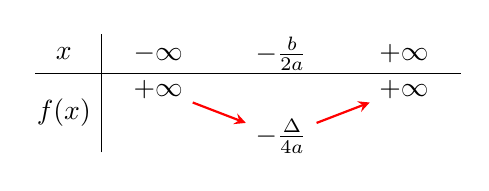
\begin{tikzpicture}[>=stealth, xscale=1.2, yscale=1]
        % Đường phân cách dòng cột
        \draw (0.5,0.5) -- (5,0.5);
        \draw (1.2, -0.5) -- (1.2, 1);
        
        % Dòng x
        \node at (0.8, 0.75) {$x$};
        \node at (1.8, 0.75) {$-\infty$};
        \node at (3.1, 0.75) {$-\frac{b}{2a}$};
        \node at (4.4, 0.75) {$+\infty$};
        
        % Dòng f(x) và các mũi tên chiều biến thiên
        \node at (0.8, 0) {$f(x)$};
        \node (y1) at (1.8, 0.3) {$+\infty$};
        \node (y2) at (3.1, -0.3) {$-\frac{\Delta}{4a}$};
        \node (y3) at (4.4, 0.3) {$+\infty$};
        
        \draw[->, red, thick] (y1) -- (y2);
        \draw[->, red, thick] (y2) -- (y3);
    \end{tikzpicture}
    &
    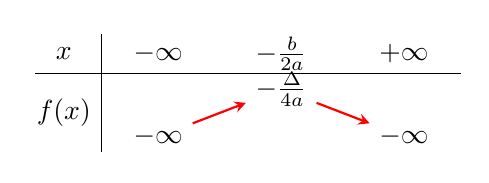
\begin{tikzpicture}[>=stealth, xscale=1.2, yscale=1]
        % Đường phân cách dòng cột
        \draw (0.5,0.5) -- (5,0.5);
        \draw (1.2, -0.5) -- (1.2, 1);
        
        % Dòng x
        \node at (0.8, 0.75) {$x$};
        \node at (1.8, 0.75) {$-\infty$};
        \node at (3.1, 0.75) {$-\frac{b}{2a}$};
        \node at (4.4, 0.75) {$+\infty$};
        
        % Dòng f(x) và các mũi tên chiều biến thiên
        \node at (0.8, 0) {$f(x)$};
        \node (y1) at (1.8, -0.3) {$-\infty$};
        \node (y2) at (3.1, 0.3) {$-\frac{\Delta}{4a}$};
        \node (y3) at (4.4, -0.3) {$-\infty$};
        
        \draw[->, red, thick] (y1) -- (y2);
        \draw[->, red, thick] (y2) -- (y3);
    \end{tikzpicture}
\end{tabular}
\end{center}
\makeheading{II}{Bài tập tự luyện}
\noindent\textbf{Câu 1:} Biểu thức nào dưới đây là tam thức bậc hai?
\begin{center}
\begin{tabular}{p{3.5cm} p{3.5cm} p{3.5cm} p{3.5cm}}
\textbf{A.} $y=1$. & \textbf{B.} $y=x$. & \textbf{C.} $y=x^2$. & \textbf{D.} $y=x^3$.
\end{tabular}
\end{center}
\noindent\textbf{Câu 2:} Với $m$ là tham số bất kì, biểu thức nào dưới đây là tam thức bậc hai?
\begin{center}
\begin{tabular}{p{3.5cm} p{3.5cm} p{3.5cm} p{3.5cm}}
\textbf{A.} $y=m$. & \textbf{B.} $y=mx$. & \textbf{C.} $y=mx^2$. & \textbf{D.} $y=x^2+m$.
\end{tabular}
\end{center}
\noindent\textbf{Câu 3:} Với $m$ là tham số bất kì, biểu thức nào dưới đây là tam thức bậc hai?
\begin{center}
\begin{tabular}{p{3.5cm} p{3.5cm} p{3.5cm} p{3.5cm}}
\textbf{A.} $y=m$. & \textbf{B.} $y=mx$. & \textbf{C.} $y=(m^2+1)x^2$. & \textbf{D.} $y=mx^2+m$.
\end{tabular}
\end{center}
\noindent\textbf{Câu 4:} Tìm tất cả các giá trị của tham số $m$ để biểu thức $f(x)=(m-2)x^2+5x+9$ là tam thức bậc hai.
\begin{center}
\begin{tabular}{p{3.5cm} p{3.5cm} p{3.5cm} p{3.5cm}}
\textbf{A.} $m \in \mathbb{R}$. & \textbf{B.} $m=2$. & \textbf{C.} $m \neq 2$. & \textbf{D.} $m \neq 0$.
\end{tabular}
\end{center}
\noindent\textbf{Câu 5:} Cho hàm số bậc hai $y=f(x)$ có đồ thị như hình bên dưới:
\begin{center}
\begin{tikzpicture}[>=stealth, scale=1.2]
    % Trục tọa độ
    \draw[->] (-1.5,0) -- (3,0) node[above] {$x$};
    \draw[->] (0,-1.8) -- (0,2.0) node[left] {$y$};
    \node[below left] at (0,0) {$O$};
    
    % Vẽ đồ thị Parabol y = 4*(x-1.5)^2 - 1
    \draw[domain=-0.2:3.2, smooth, variable=\x, blue, thick] plot ({\x}, {4*(\x-1.5)^2 - 1});
    
    % Đường nét đứt
    \draw[dashed] (1.5,-1) -- (0,-1);
    \node[left] at (0,-1) {$-1$};
    
    % Các điểm trên trục hoành
    \filldraw (1,0) circle (1pt) node[above left] {$1$};
    \filldraw (2,0) circle (1pt) node[above left] {$2$};
\end{tikzpicture}
\end{center}
Khẳng định nào dưới đây đúng?
\begin{center}
\begin{tabular}{p{7.5cm} p{7.5cm}}
\textbf{A.} $f(x)>0, \forall x \in (0;2)$. & \textbf{B.} $f(x)<0, \forall x \in (0;2)$. \\
\textbf{C.} $f(x)>0, \forall x \in (1;+\infty)$. & \textbf{D.} $f(x)<0, \forall x \in (1;2)$.
\end{tabular}
\end{center}
\noindent\textbf{Câu 6:} Tam thức bậc hai nào dưới đây có bảng xét dấu như hình vẽ?
\begin{center}
\begin{tabular}{|c|ccccccc|}
\hline
$x$ & $-\infty$ & & $0$ & & $4$ & & $+\infty$ \\
\hline
$f(x)$ & & $+$ & $0$ & $-$ & $0$ & $+$ & \\
\hline
\end{tabular}
\end{center}
\begin{center}
\begin{tabular}{p{3.5cm} p{3.5cm} p{3.5cm} p{3.5cm}}
\textbf{A.} $y=x^2-2x$. & \textbf{B.} $y=x^2+2x$. & \textbf{C.} $y=x^2-4x$. & \textbf{D.} $y=-x^2+4x$.
\end{tabular}
\end{center}
\noindent\textbf{Câu 7:} Tam thức bậc hai nào dưới đây có bảng xét dấu như hình vẽ?
\begin{center}
\begin{tabular}{|c|ccccccc|}
\hline
$x$ & $-\infty$ & & $0$ & & $2$ & & $+\infty$ \\
\hline
$f(x)$ & & $-$ & $0$ & $+$ & $0$ & $-$ & \\
\hline
\end{tabular}
\end{center}
\begin{center}
\begin{tabular}{p{3.5cm} p{3.5cm} p{3.5cm} p{3.5cm}}
\textbf{A.} $y=x^2-2x$. & \textbf{B.} $y=-x^2+2x$. & \textbf{C.} $y=x^2-4x$. & \textbf{D.} $y=x^2+4x$.
\end{tabular}
\end{center}
\noindent\textbf{Câu 8:} Cho tam thức $f(x)=x^2-3x+2$. Khẳng định nào dưới đây đúng?
\begin{center}
\begin{tabular}{p{7.5cm} p{7.5cm}}
\textbf{A.} $f(x)>0, \forall x \in (1;2)$. & \textbf{B.} $f(x)<0, \forall x \in (1;2)$. \\
\textbf{C.} $f(x)<0, \forall x \in (-\infty;1) \cup (2;+\infty)$. & \textbf{D.} $f(x)<0, \forall x \in [1;2]$.
\end{tabular}
\end{center}
\noindent\textbf{Câu 9:} Cho tam thức $f(x)=x^2-3x+2$. Khẳng định nào dưới đây \textbf{sai}?
\begin{center}
\begin{tabular}{p{7.5cm} p{7.5cm}}
\textbf{A.} $f(x)>0, \forall x \in (-\infty;1) \cup (2;+\infty)$. & \textbf{B.} $f(x)<0, \forall x \in (1;2)$. \\
\textbf{C.} $f(x)>0, \forall x \in (-\infty;1] \cup [2;+\infty)$. & \textbf{D.} $f(x) \leq 0, \forall x \in [1;2]$.
\end{tabular}
\end{center}
\noindent\textbf{Câu 10:} Tập hợp tất cả các giá trị của $x$ để tam thức $y=-x^2+2x$ luôn âm là:
\begin{center}
\begin{tabular}{p{7.5cm} p{7.5cm}}
\textbf{A.} $(0;2)$. & \textbf{B.} $(-\infty;0) \cup (2;+\infty)$. \\
\textbf{C.} $[0;2]$. & \textbf{D.} $(-\infty;0] \cup [2;+\infty)$.
\end{tabular}
\end{center}
\makeheading{III}{Bài tập làm thêm}
\noindent\textbf{Câu 11:} Tập hợp tất cả các giá trị của $x$ để tam thức $f(x)=x^2-2x$ luôn dương là
\begin{center}
\begin{tabular}{p{3.5cm} p{3.5cm} p{3.5cm} p{3.5cm}}
\textbf{A.} $(0;2)$. & \textbf{B.} $(-\infty;0) \cup (2;+\infty)$. & \textbf{C.} $[0;2]$. & \textbf{D.} $(-\infty;0] \cup [2;+\infty)$.
\end{tabular}
\end{center}
\noindent\textbf{Câu 12:} Tam thức nào dưới đây luôn âm với mọi $x \in \mathbb{R}$?
\begin{center}
\begin{tabular}{p{3.5cm} p{3.5cm} p{3.5cm} p{3.5cm}}
\textbf{A.} $y=x^2+x+1$. & \textbf{B.} $y=-x^2+x+1$. & \textbf{C.} $y=-x^2+x-1$. & \textbf{D.} $y=-x^2+4x$.
\end{tabular}
\end{center}
\noindent\textbf{Câu 13:} Tam thức nào dưới đây luôn dương với mọi $x \in \mathbb{R}$?
\begin{center}
\begin{tabular}{p{3.5cm} p{3.5cm} p{3.5cm} p{3.5cm}}
\textbf{A.} $y=x^2+x+1$. & \textbf{B.} $y=x^2-2x+1$. & \textbf{C.} $y=-x^2+x-1$. & \textbf{D.} $y=-x^2+4x$.
\end{tabular}
\end{center}
\noindent\textbf{Câu 14:} Một nghiệm của bất phương trình $x^2-2x-3>0$ là
\begin{center}
\begin{tabular}{p{3.5cm} p{3.5cm} p{3.5cm} p{3.5cm}}
\textbf{A.} $x=5$. & \textbf{B.} $x=0$. & \textbf{C.} $x=-2$. & \textbf{D.} $x=4$.
\end{tabular}
\end{center}
\noindent\textbf{Câu 15:} Tập nghiệm của bất phương trình $x^2-2x-3>0$ là
\begin{center}
\begin{tabular}{p{3.5cm} p{3.5cm} p{3.5cm} p{3.5cm}}
\textbf{A.} $[-1;3]$. & \textbf{B.} $(-\infty;-1) \cup (3;+\infty)$. & \textbf{C.} $(-1;3)$. & \textbf{D.} $(-\infty;-1] \cup [3;+\infty)$.
\end{tabular}
\end{center}
\noindent\textbf{Câu 16:} Tập nghiệm của bất phương trình $x^2-2x-3\ge 0$ là
\begin{center}
\begin{tabular}{p{3.5cm} p{3.5cm} p{3.5cm} p{3.5cm}}
\textbf{A.} $[-1;3]$. & \textbf{B.} $(-\infty;-1) \cup (3;+\infty)$. & \textbf{C.} $(-1;3)$. & \textbf{D.} $(-\infty;-1] \cup [3;+\infty)$.
\end{tabular}
\end{center}
\noindent\textbf{Câu 17:} Tập nghiệm của bất phương trình $x^2-2x-3\le 0$ là
\begin{center}
\begin{tabular}{p{3.5cm} p{3.5cm} p{3.5cm} p{3.5cm}}
\textbf{A.} $[-1;3]$. & \textbf{B.} $(-\infty;-1) \cup (3;+\infty)$. & \textbf{C.} $(-1;3)$. & \textbf{D.} $(-\infty;-1] \cup [3;+\infty)$.
\end{tabular}
\end{center}
\noindent\textbf{Câu 18:} Tập nghiệm của bất phương trình $x^2-2x+3>0$ là
\begin{center}
\begin{tabular}{p{3.5cm} p{3.5cm} p{3.5cm} p{3.5cm}}
\textbf{A.} $\varnothing$. & \textbf{B.} $\mathbb{R}$. & \textbf{C.} $(1;3)$. & \textbf{D.} $(-\infty;-1] \cup [3;+\infty)$.
\end{tabular}
\end{center}
\noindent\textbf{Câu 19:} Tập nghiệm của bất phương trình $x^2-x+3\ge 0$ là
\begin{center}
\begin{tabular}{p{3.5cm} p{3.5cm} p{3.5cm} p{3.5cm}}
\textbf{A.} $\varnothing$. & \textbf{B.} $\mathbb{R}$. & \textbf{C.} $(1;3)$. & \textbf{D.} $(-\infty;-1] \cup [3;+\infty)$.
\end{tabular}
\end{center}
\noindent\textbf{Câu 20:} Tập nghiệm của bất phương trình $x^2-x+3<0$ là
\begin{center}
\begin{tabular}{p{3.5cm} p{3.5cm} p{3.5cm} p{3.5cm}}
\textbf{A.} $\varnothing$. & \textbf{B.} $\mathbb{R}$. & \textbf{C.} $(1;3)$. & \textbf{D.} $(-\infty;-1] \cup [3;+\infty)$.
\end{tabular}
\end{center}
\end{document}